\chapter{The LHC and the CMS Detector}
\label{detector}
\section{The LHC}
The Large Hadron Collider (LHC) at CERN is currently the leading collider experiment designed 
to study physics at the TeV scale. The collider is an octagonal 
ring, 27 km in circumference, hosted in the former LEP tunnel in France/Switzerland.  
Both proton-proton (p-p) and heavy ion (Pb-Pb) collisions are
studied as part of the LHC physics programme however, the former are used 
for direct searches for new physics. Proton beams are formed inside the proton synchrotron (PS)
from bunches of protons 50 ns apart with an energy of 26 GeV. The protons are then accelerated in the 
super proton synchrotron (SPS) to 450 GeV before being injected into the LHC. 
Around 1200 superconducting dipole magnets maintain two beams of protons accelerating around 
the ring in opposite directions before being collided at one of the four major experiments;
Atlas, CMS, LHCb and ALICE.
Figure~\ref{fig:lhcring} is a cartoon of the accelerator indicating the sites of the
four experiments.

\begin{figure}[htb!]
\begin{center}
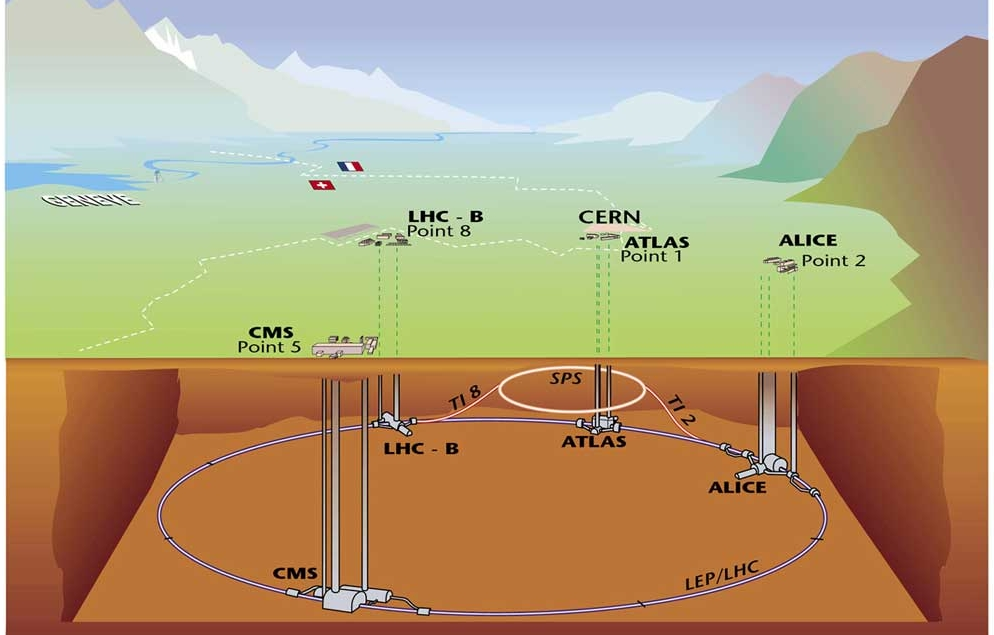
\includegraphics[width=0.8\textwidth]{detector/CERN.jpg}
\caption{LHC accelerator ring. The relative locations of the four main experiments 
are indicated along with their points of access to the beam.}
\label{fig:lhcring}
\end{center}
\end{figure}

The first major physics runs began in May 2010 with a centre of mass energy 
$\sqrt{s}=7~TeV$ and continued until November providing a $44pb^{-1}$ integrated luminosity of data.
The LHC resumed collisions in April 2011 delivering a further $6fb^{-1}$ by the end
of October. The centre of mass energy was increased to $\sqrt{s}=8~TeV$ for the 2012 p-p 
collision run, improving the sensitivity of searches for new physics. A total of
$6fb^{-1}$ of 8 TeV data were taken by July 2012 which were combined with earlier data resulting
in the discovery of a new boson reported by CMS and Atlas at the ICHEP conference that year. 

\section{The CMS Detector}
\label{cmsdetector}
The Compact Muon Solenoid (CMS) detector is one of two general purpose detectors at 
the LHC designed to search for new physics. 
Among the wide range of physics programs at CMS, the search for the SM Higgs boson 
has a high priority. The decay rates of the SM Higgs boson in different 
channels vary dramatically as a function of its mass ($\mh$). A key feature of the experiment's design
was therefore the necessity to maintain a high sensitivity to the SM Higgs for a wide range of masses in as many 
decay channels as possible. To achieve this, several detector components are layered around 
the beam axis reconstruct almost any known particle produced at the interaction point.
Each component consists of a cylindrical barrel section and two endcaps 
to provide an almost hermetic coverage of the outgoing particle flux.


The tracker, providing measurements of the momentum of charged particles and the location of 
primary and secondary vertices (from decays of heavy flavour mesons), is the first layer of detection.
This is followed by the electromagnetic calorimeter (ECAL) which is used to measure
the energy deposited as electromagnetic showers from interacting electrons and photons. 
The hadronic calorimeter (HCAL) complements this by providing energy measurements of 
sprays of hadrons, known as jets, which deposit energy through nuclear interactions. 
The HCAL is a sampling calorimeter in that the active material (plastic scintillators)
are sandwiched between dense absorbing material to increase the depth of the calorimeter to
around 11 radiation lengths. The addition of the forward calorimeter (HF) extends the HCAL
coverage to roughly $|\eta|=5$.  
The tracker and calorimeters are situated within a 4T axial magnetic field 
provided by the superconducting magnet surrounding them.
The magnetic flux return is implemented within the  muon detector systems which lie outside 
the superconducting coil and form the outermost detection layers. Muons deposit very little energy 
throughout the detector and can carry on into the surrounding cavern.
The barrel muon system is constructed from layers of drift-tubes (DT) interleaved with 
resistive plate chambers. The combination of the two provides high resolution
timing and hit positions which are used to determine the trajectory of muons both from
p-p collisions and cosmic sources for calibration. For the endcaps, the DTs are replaced
with cathode strip chambers as the higher flux of particles along the beam line
requires the use of radiation hard components.
% ------------------------------------------------------------------------------------

CMS uses a Cartesian coordinate system with the origin at the 
interaction point and the $z$-axis pointing along the beam axis. The $x$-axis points towards 
the centre of the LHC ring and the $y$-axis points vertically upwards. The azimuthal angle, 
$\phi~\epsilon~[-\pi,\pi]$, is defined with respect to the $x$-axis in the in the 
transverse ($x-y$) plane. The polar angle $\theta$ is measured from the $z$-axis. Commonly,
the direction of an outgoing particle is defined by $\phi$ and its pseudo-rapidity $\eta$ 
defined as 
\begin{equation}
	\eta=-\log \tan \left( \frac{\theta}{2} \right).
\end{equation}
As hard collisions produce high momentum particles travelling perpendicular to the beam line, 
particles are often characterised
by the magnitude of the projection of their momenta onto the transverse plane, 
$\pt=\sqrt{p_{x}^{2}+p_{y}^{2}}$.
Similarly, the transverse energy is defined as $E_{T}=E\sin\theta$.
Figure~\ref{fig:cms} shows the geometry of the CMS detector and its major components. 

\begin{figure}
\centering
	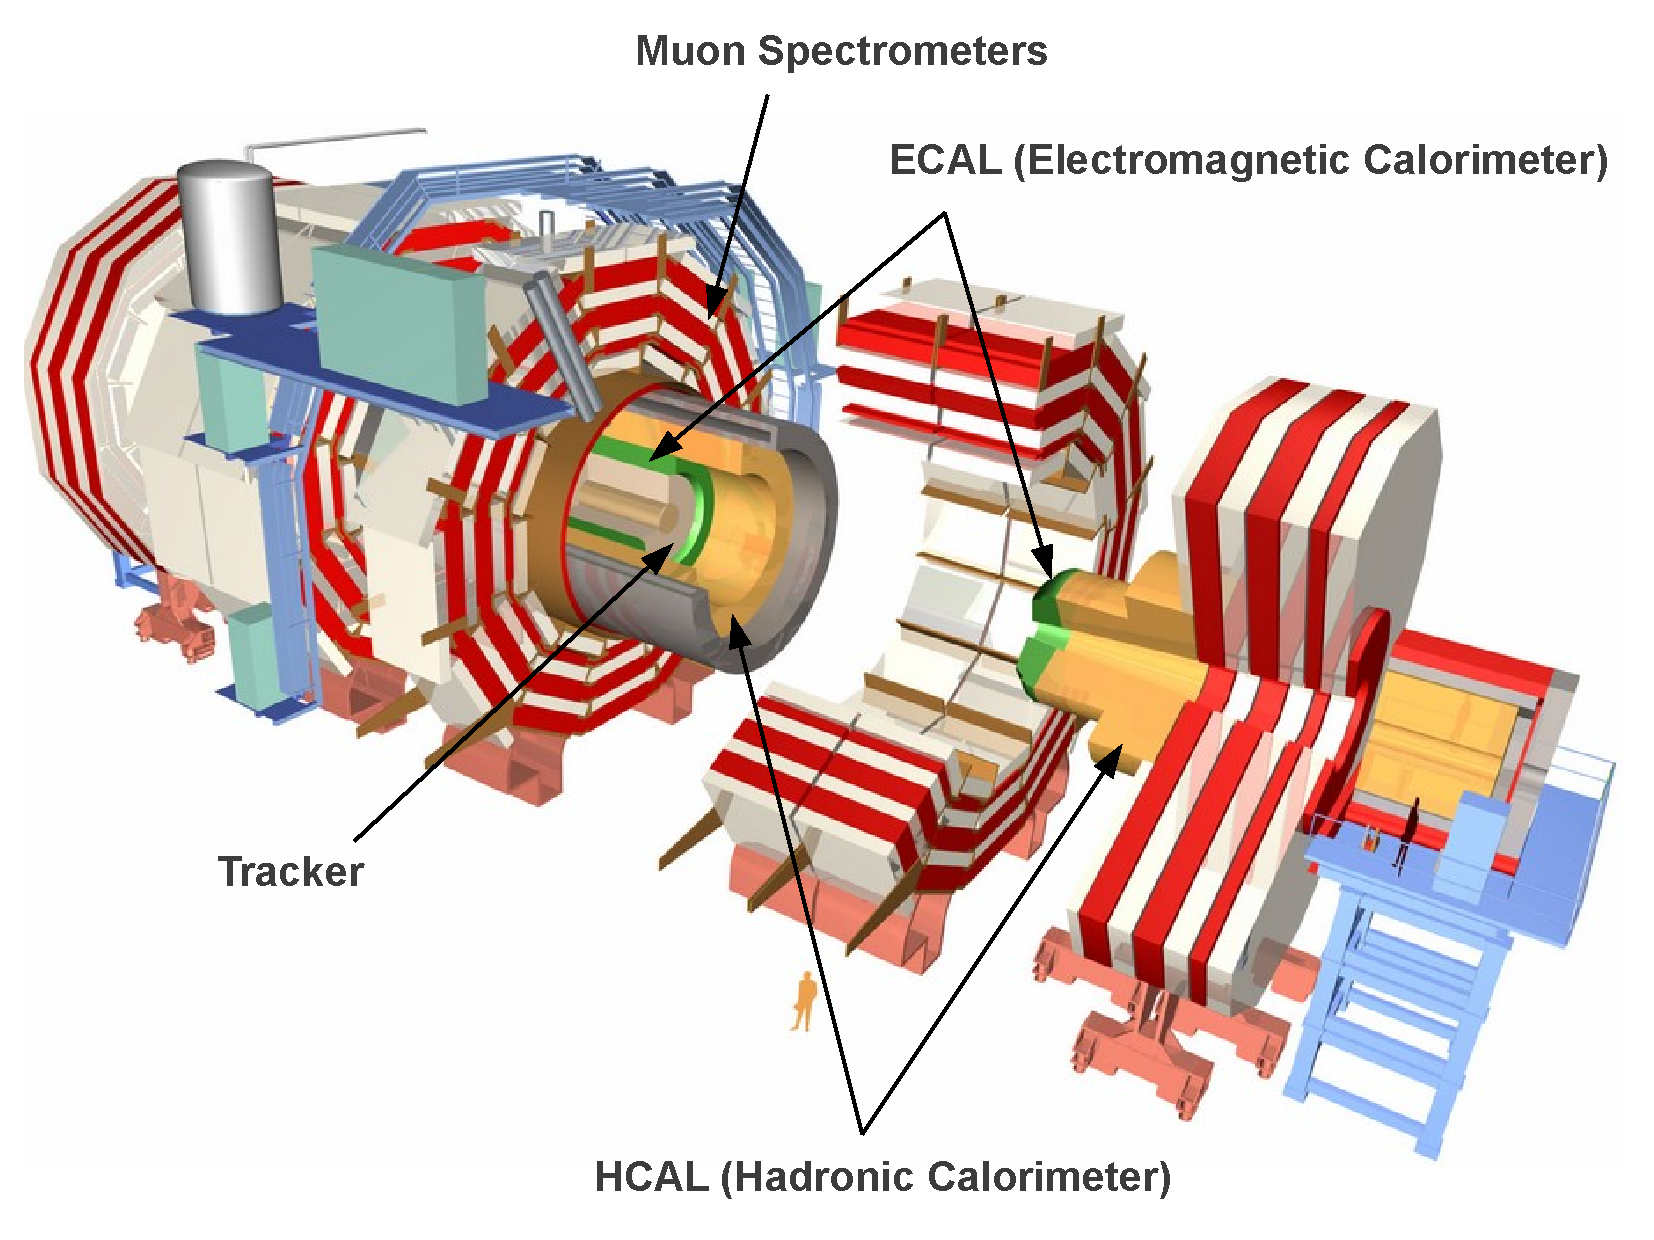
\includegraphics[width=0.8\textwidth]{detector/cmsdetector}
	\caption{Diagram of the CMS Detector. The arrows indicate the main detector elements. 
	The figure has been altered from its original source~\cite{cmspub}}
	\label{fig:cms}
\end{figure}

\subsection{Tracker}
The CMS tracker is designed to reconstruct charged particle tracks 
which make up a large portion of the complex topology of 
p-p collisions. The tracker provides precise measurements of 
observables such as the momentum of charged particles and the location of the
vertex at which they are produced.
In addition to the high level of granularity required to make such measurements, the 
high rate of interaction at LHC requires a fast response from the tracking 
elements. 
The tracker is formed of a pixel detector component encased by layers of silicon strip detectors.
The pixel detector is the closest tracking element to the interaction point. 
It is a composite of 66 million individual silicon pixels, $100\mu m \times 150 \mu m$ in size,
forming three cylindrical layers around the beam line and two forward disks. 
%The resolution of the pixel detector is around 10 $\mathrm{\mu}$m in the $\hat{r}$ and $\hat{\phi}$ 
%direction and 17 $\mathrm{\mu}$m in $\hat{z}$%~\cite{trckAC}. 
Outside the pixel detector, ten cylindrical layers of silicon strip detectors (TIB/TOB) 
and twelve discs (TID/TEC) extend the tracking system out to a radius of 120cm from the 
beam line. The tracker geometry, as shown in Figure~\ref{fig:trackergeom}, covers a pseudo-rapidity 
range $|\eta| < 2.5$.

\begin{figure}
	\centering
	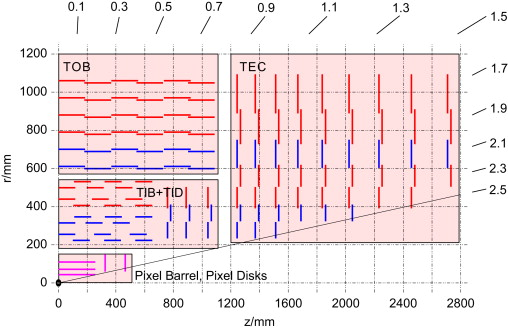
\includegraphics[width=0.9\textwidth]{detector/trcker/tracker_col.jpg}
	\caption{Cross-section of the pixel and silicon strip detector 
	components of the CMS tracker~\cite{Weber201159}.}
   \label{fig:trackergeom}
\end{figure}

By making multiple precise measurements throughout the tracker system,the trajectories (tracks) of charged 
particles can be reconstructed.
Tracks are associated to a common point of origin (primary vertex) by grouping those which are separated
by less than 1cm in the $z$ coordinate of the point of closest approach to the beam line.
The vertex resolution is dependant both on the number of tracks associated to the vertex and
their average transverse momenta ($\bar{p_{T}}$). The resolution was measured in early data from 2010
by splitting tracks associated to a vertex randomly into two groups with equal kinematic distributions.
The difference between the vertex locations calculated from the two groups was used to provide an estimate 
of the resolution~\cite{TRK-10-005}.
Figure~\ref{fig:vtxreso} shows the resolution in $z$ as a function of the track multiplicity
measured in data and simulation. The simulation provides a good description of both the trend with 
number of associated tracks and the improvement in resolution with $\bar{p_{T}}$ in the data. 

\begin{figure}
\begin{center}
	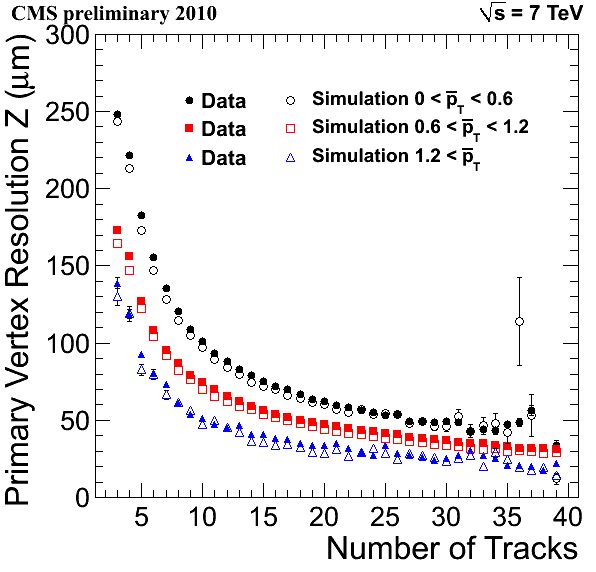
\includegraphics[width=.6\textwidth]{detector/trcker/zresotrcker.png}
	\caption{Resolution of vertex $z$-position as a function of the number 
	of tracks associated to the vertex measured in simulation and 2010 data.
 	The resolution is given for three different average track momenta.}
	\label{fig:vtxreso}
\end{center}
\end{figure}

\subsection{Electromagnetic Calorimeter}
The electromagnetic calorimeter (ECAL) is used to reconstruct the energies of electromagnetically 
interacting particles such as electrons and photons. 
It is constructed from high density lead tungstate (PbWO$_{4}$) crystals which
form a barrel section (EB) and two endcaps (EE) outside the tracker. 
Two lead plates in front of a fine grained silicon strip detector are situated just before the 
endcaps forming the ECAL pre-shower (PS). 
Photons travelling at high $\eta$ will convert in the lead and the resulting electron-positron pair
will produce tracks which can be used to pinpoint the position of the incoming photon. This additional
resolution in spatial separation can be used to distinguish prompt photons from those produced
in neutral pion decays.

The ECAL is designed to cover a pseudo-rapidity range of $|\eta | < 3$. 
The crystals are arranged to form modules which surround the beam line in a `non-projective geometry':
the gaps between crystal modules are offset by 3$^{\circ}$ with respect to particle trajectories originating from 
the interaction point. Electrons and photons deposit most of their energy within 
the crystals as the depth of the crystals is equivalent to 25.8 radiation lengths~\cite{TDR1}. 
Electromagnetic showers produced by the interaction of electrons and photons in the ECAL crystals
produce scintillation light which is collected to measure the energy of the particle. 
The scintillation output of the crystals is, however, low and temperature dependant 
($\sim$ 2.1\%/K at the ECAL operating temperature of 291 K). 
To overcome this low yield, avalanche photo-diodes (APD's) and vacuum 
photo-triodes (VPT's) are used to collect the scintillation light and amplify the signal in the 
calorimeter barrel and endcaps respectively. Around 4.5 photo-electrons per MeV are produced in both 
APD's and VPT's. 
%Around 80\% of the scintillation light produced in electromagnetic particles is collected during the 

\subsubsection{Electron and Photon Reconstruction}

Electron and photon candidates are formed by clustering deposits of 
energy caused by electromagnetic showers in the ECAL. For unconverted 
photons, these clusters will likely be well localised in $\eta$ and $\phi$
around the incident photon. However, for photons which convert in the tracker,
the resulting electron-positron pair will deposit energy across several regions
of the calorimeter. In the presence of the axial magnetic field, 
electrons radiate bremsstrahlung photons causing deposits which are 
spread over a wide range in $\phi$ while being fairly narrow in $\eta$.
This characteristic is exploited by the ``Hybrid'' clustering algorithm 
used to reconstruct high energy electrons and photons in
the ECAL barrel~\cite{cseez}. The algorithm proceeds as follows;
\begin{itemize}
 \item Step 1: A seed crystal is determined to be a single crystal in the barrel with the highest
 $E_{T}$ satisfying $E_{T}>1~GeV$.
 \item Step 2: $1\times3$ ($\phi\times\eta$) crystal dominoes are formed with their central crystal 
 aligned with the seed crystal in $\eta$. If the energy contained in the $1\times3$ domino is 
 larger than 1 GeV, the domino is extended by two crystals in $\eta$. A maximum of 10 dominoes are 
 added in each direction in $\phi$ starting from the seed crystal forming a sub-cluster.
 \item Step 3: Dominoes containing less than 100 MeV are removed and the remaining dominoes are 
 grouped into sub-clusters providing each seeding domino for a sub-cluster contains more than 350 MeV. 
 The final group of sub-clusters form a supercluster for the electromagnetic object.
\end{itemize}
The values of the particular thresholds used for seeding clusters and dominoes were tuned providing
an efficiency for electrons with $p_{T}>7~GeV$ greater than 99\%~\cite{dfutyan}.
Figure~\ref{fig:hybridclustering} is an illustration of the Hybrid clustering algorithm.

\begin{figure}
\begin{center}
	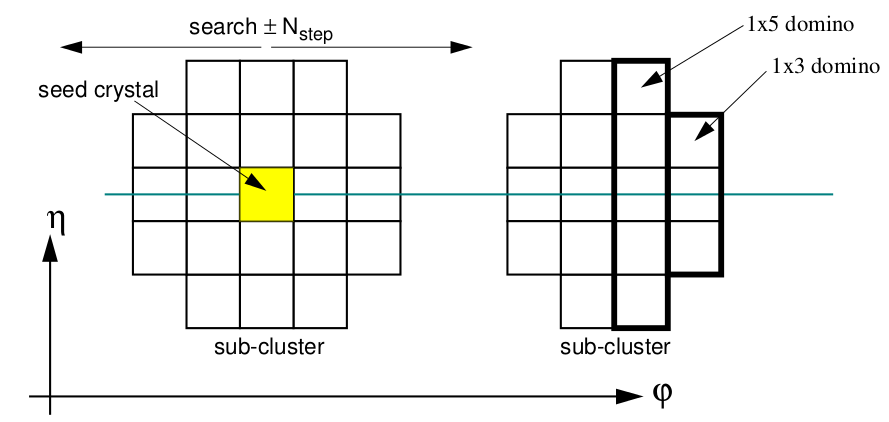
\includegraphics[width=0.8\textwidth]{detector/ecal/clustering.png}
	\caption{Sub-cluster construction of the Hybrid algorithm used to reconstruct photons and 
	electrons in the ECAL barrel.}
	\label{fig:hybridclustering}
\end{center}
\end{figure}

In the ECAL endcaps, superclusters are built using the ``Island'' algorithm which connects
rows of crystals whose energy decrease monotonically from the central seed crystal~\cite{cseez}.
The flat geometry of the endcaps does not allow for the in-built bremsstrahlung recovery
of the Hybrid algorithm used in the barrel. Additional information is used from the PS to enhance the 
energy reconstruction in the endcaps. 

Superclusters are associated to electron candidates (\texttt{GsfElectrons}) 
where a track can be reconstructed from
compatible hits in the tracker using a Gaussian sum filter algorithm~\cite{GSF_Electron_Reconstruction_CMS}.  
This provides an additional measure of the electron's momentum which is used 
to improve the resolution of the electron energy.
Aside from this, the reconstruction of photons and electrons is identical which is an 
important feature allowing for data driven calibrations and validations of photons using 
electrons such as those described in Chapter~\ref{chap:hgg}.


\subsubsection{Laser Calibration}

ECAL crystals suffer from loss of optical transmission when irradiated through 
the formation of crystal-lattice defaults which absorb some of the scintillation light. Annealing
acts to balance the damage from radiation which results in an equilibrium optical 
transmission which is dose-dependant~\cite{TDR1}. 
At the LHC, the dose varies during each run. This requires that the time varying optical transmission of the ECAL 
crystals be monitored to asses the impact on energy measurements.
The crystal transparency is monitored by comparing the relative transmission in blue laser light (440 nm), 
which is close to the scintillation emission peak, to infra-red (796 nm), which is far from the 
peak and relatively unaffected by the radiation damage.
Figure~\ref{fig:trans} shows the relative response to the blue laser of the monitoring system
averaged over all the crystals in bins of $|\eta|$ throughout the 2011 data taking 
runs~\cite{CMS-DP-2012-007}. 
The time dependence of the response has larger variation for higher values of $|\eta|$ due to the larger flux
of particles along the beam axis.

\begin{figure}
	\centering
	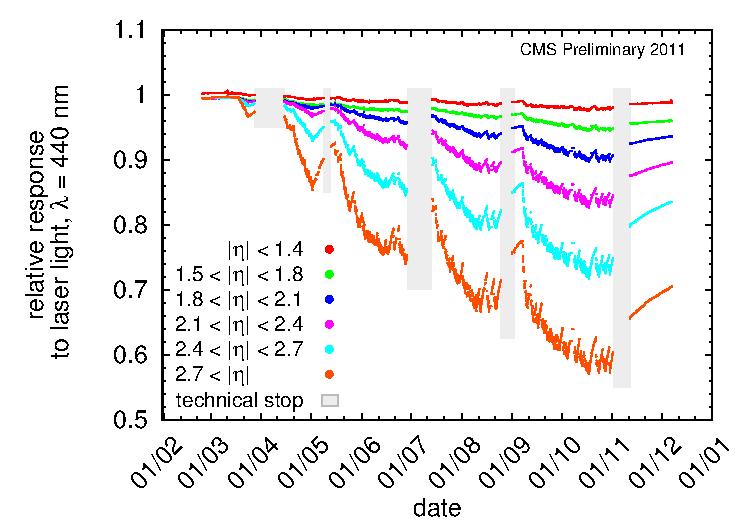
\includegraphics[width=0.8\textwidth]{detector/ecal/laser.pdf}
	\caption{Relative ECAL crystal response to blue laser light (440 nm) in bins of pseudorapidity, 
	for the 2011 data taking period runs. The grey bands indicate periods during which there was no beam.}
	\label{fig:trans}
\end{figure}

The response of the crystals measured using the laser monitoring system is used to calibrate 
the energy reconstruction of the ECAL. These calibrations are validated in $W\rightarrow e\nu$ data events
by comparing the electron energy ($E$) measured as measured by the ECAL to the momentum 
($p$) of the electron measured in the tracker~\cite{CMS-DP-2012-007}. 
Figure~\ref{fig:scaleeop} shows the relative variation in the ratio $E/p$ as a function of time 
throughout 2011. A stable scale is achieved through application of the laser calibrations.

\begin{figure}
	\centering
	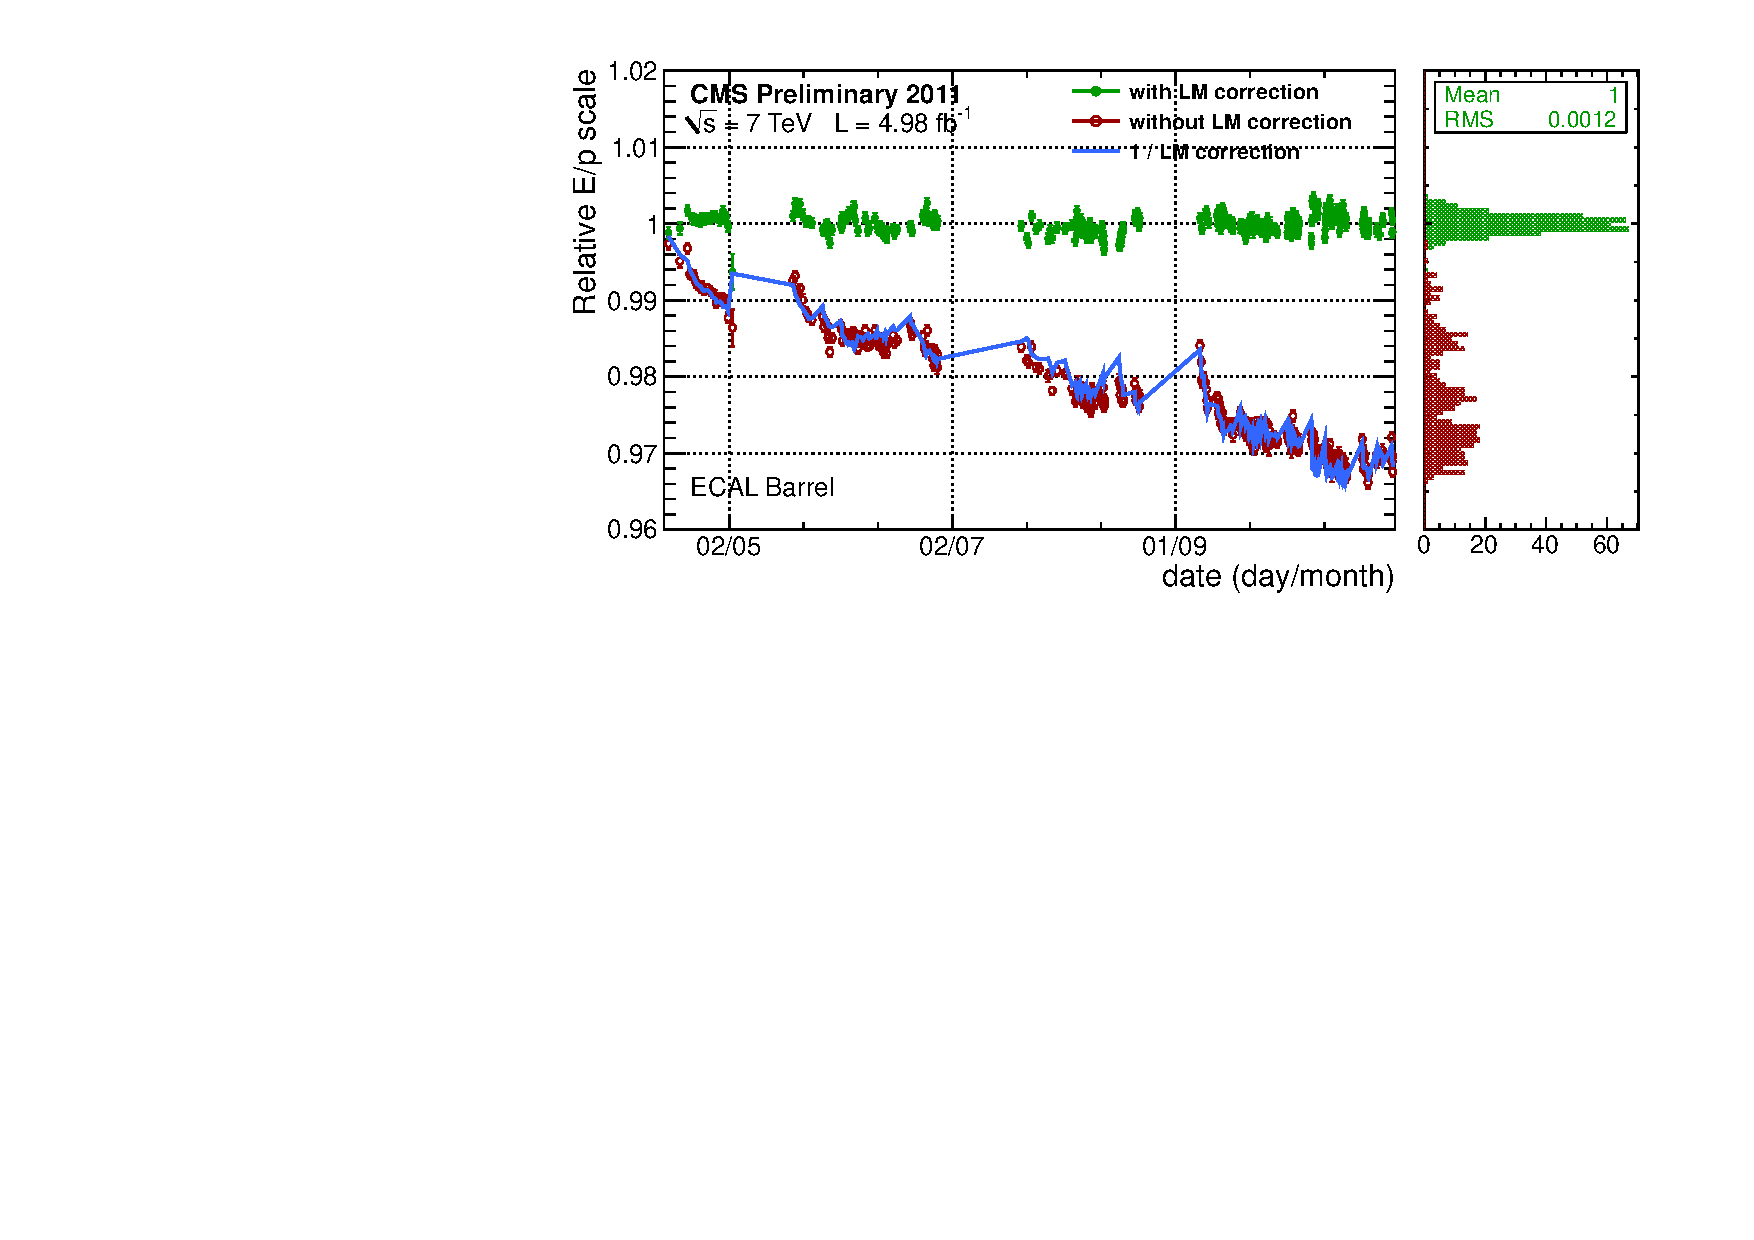
\includegraphics[width=\textwidth]{detector/ecal/scaleeop.pdf}
	\caption{Ratio $E/p$ in electrons reconstructed in the ECAL Barrel 
	from $W\rightarrow e\nu$ events in 2011 data as a function of time before 
	and after applying transparency corrections from the laser monitoring (LM) system. 
	The blue line indicates the correction applied per point averaged over all crystals used in the electron
	energy measurement.}
	\label{fig:scaleeop}
\end{figure}

\subsection{Shower-shape and Isolation}
In addition to providing a measurement of the energy of incoming electromagnetic particles,
the ECAL's fine granularity provides additional information which can be used to characterise
the supercluster and distinguish prompt electrons and photons from fakes.  
The shape of the electromagnetic shower can be described by the ratio of the energy contained
in the central $3\times3$ cluster surrounding the seed crystal to the total energy of the supercluster
($\rnine$). Superclusters associated to real unconverted photons will typically have larger value of 
$\rnine$ than those which are in reality due narrow $\pi^{0}$ decays. Another common variable used
for identification is the energy weighted crystal width of the sub-cluster used to seed the supercluster,
$\sigieie$. Prompt photons will tend to have a more localised cluster leading to lower values of $\sigieie$. 
The distributions of $\rnine$ and $\sigieie$ are shown for a simulated sample of 
superclusters identified as photons from real and fake sources in Figure~\ref{fig:showershape}.
The two distinct peaks in the $\sigieie$ distribution are due to the different superclustering algorithms 
used in the barrel and endcaps.

\begin{figure}[hbt!]
\begin{center}
	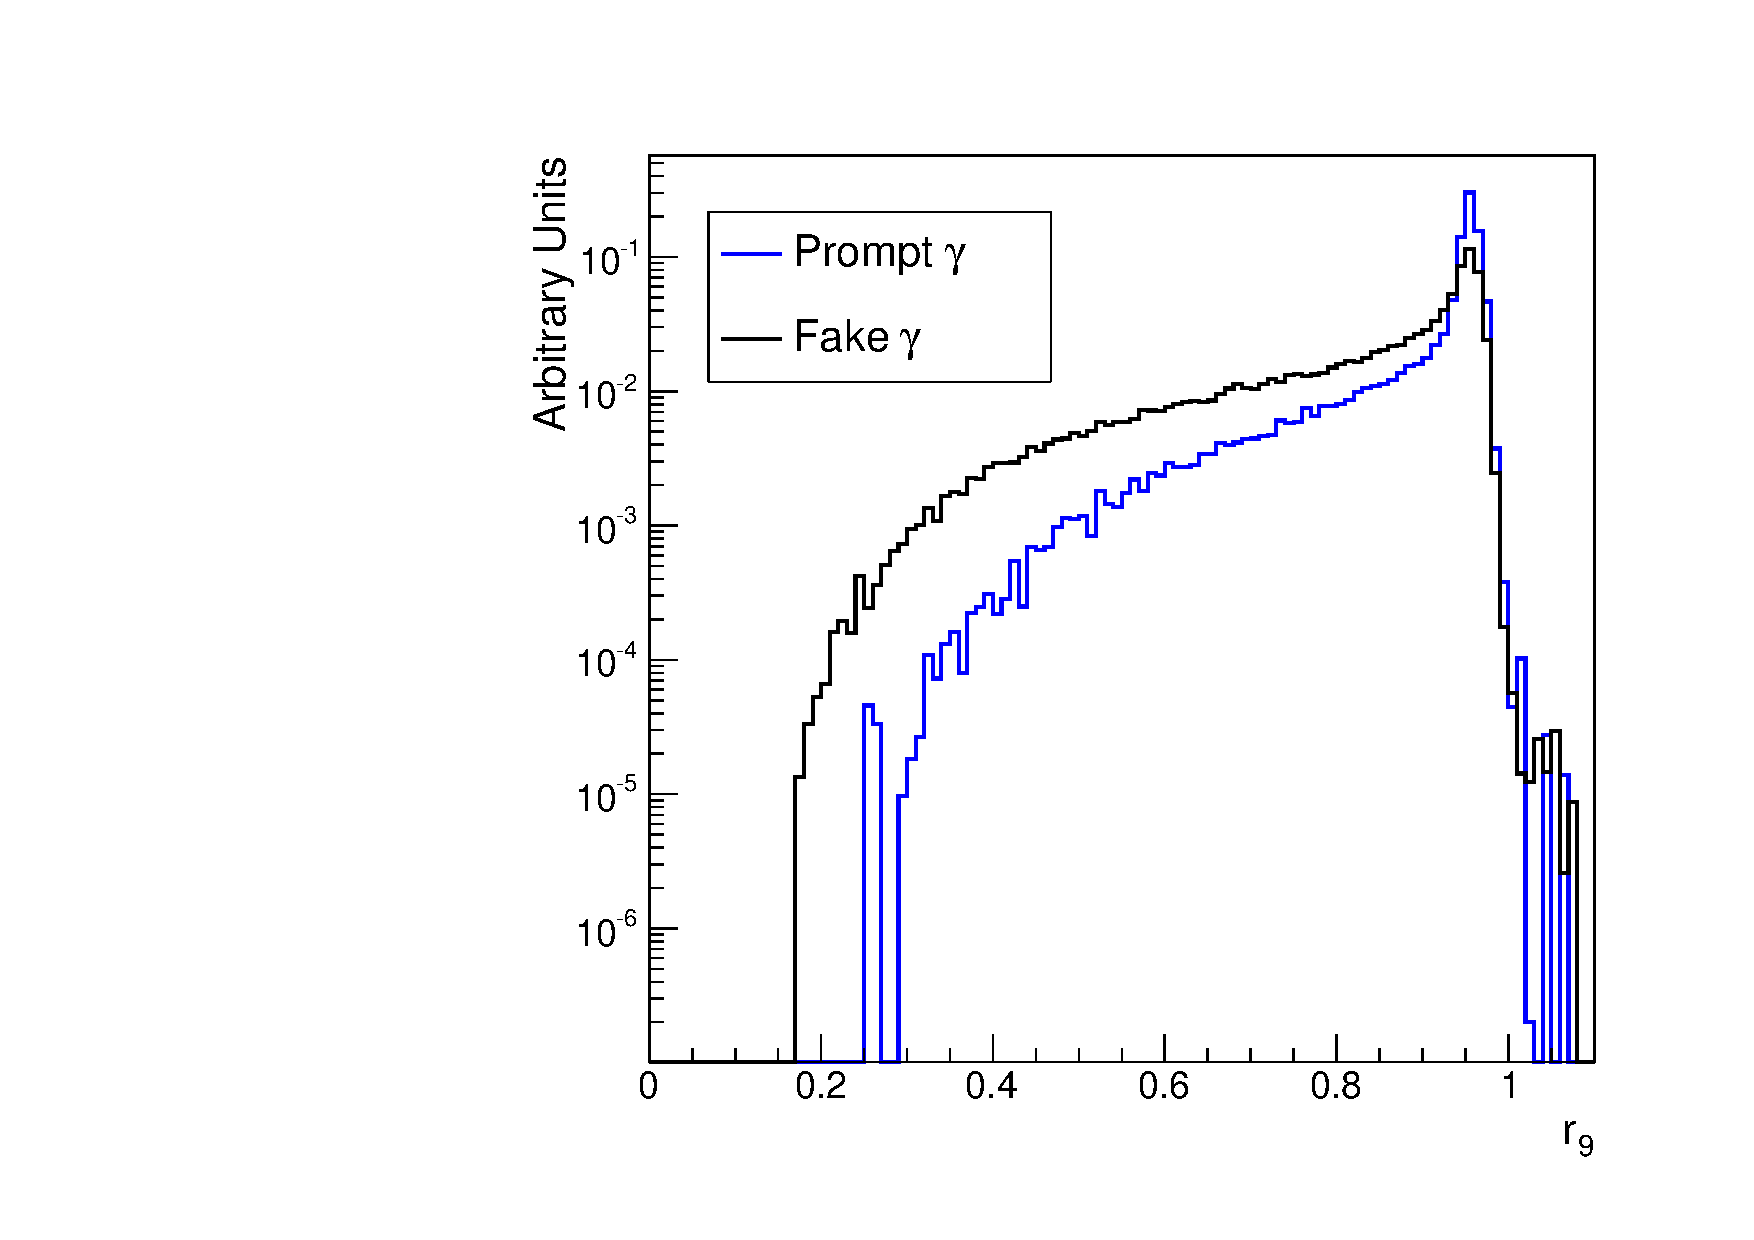
\includegraphics[width=0.49\textwidth]{detector/r9eg.pdf}
	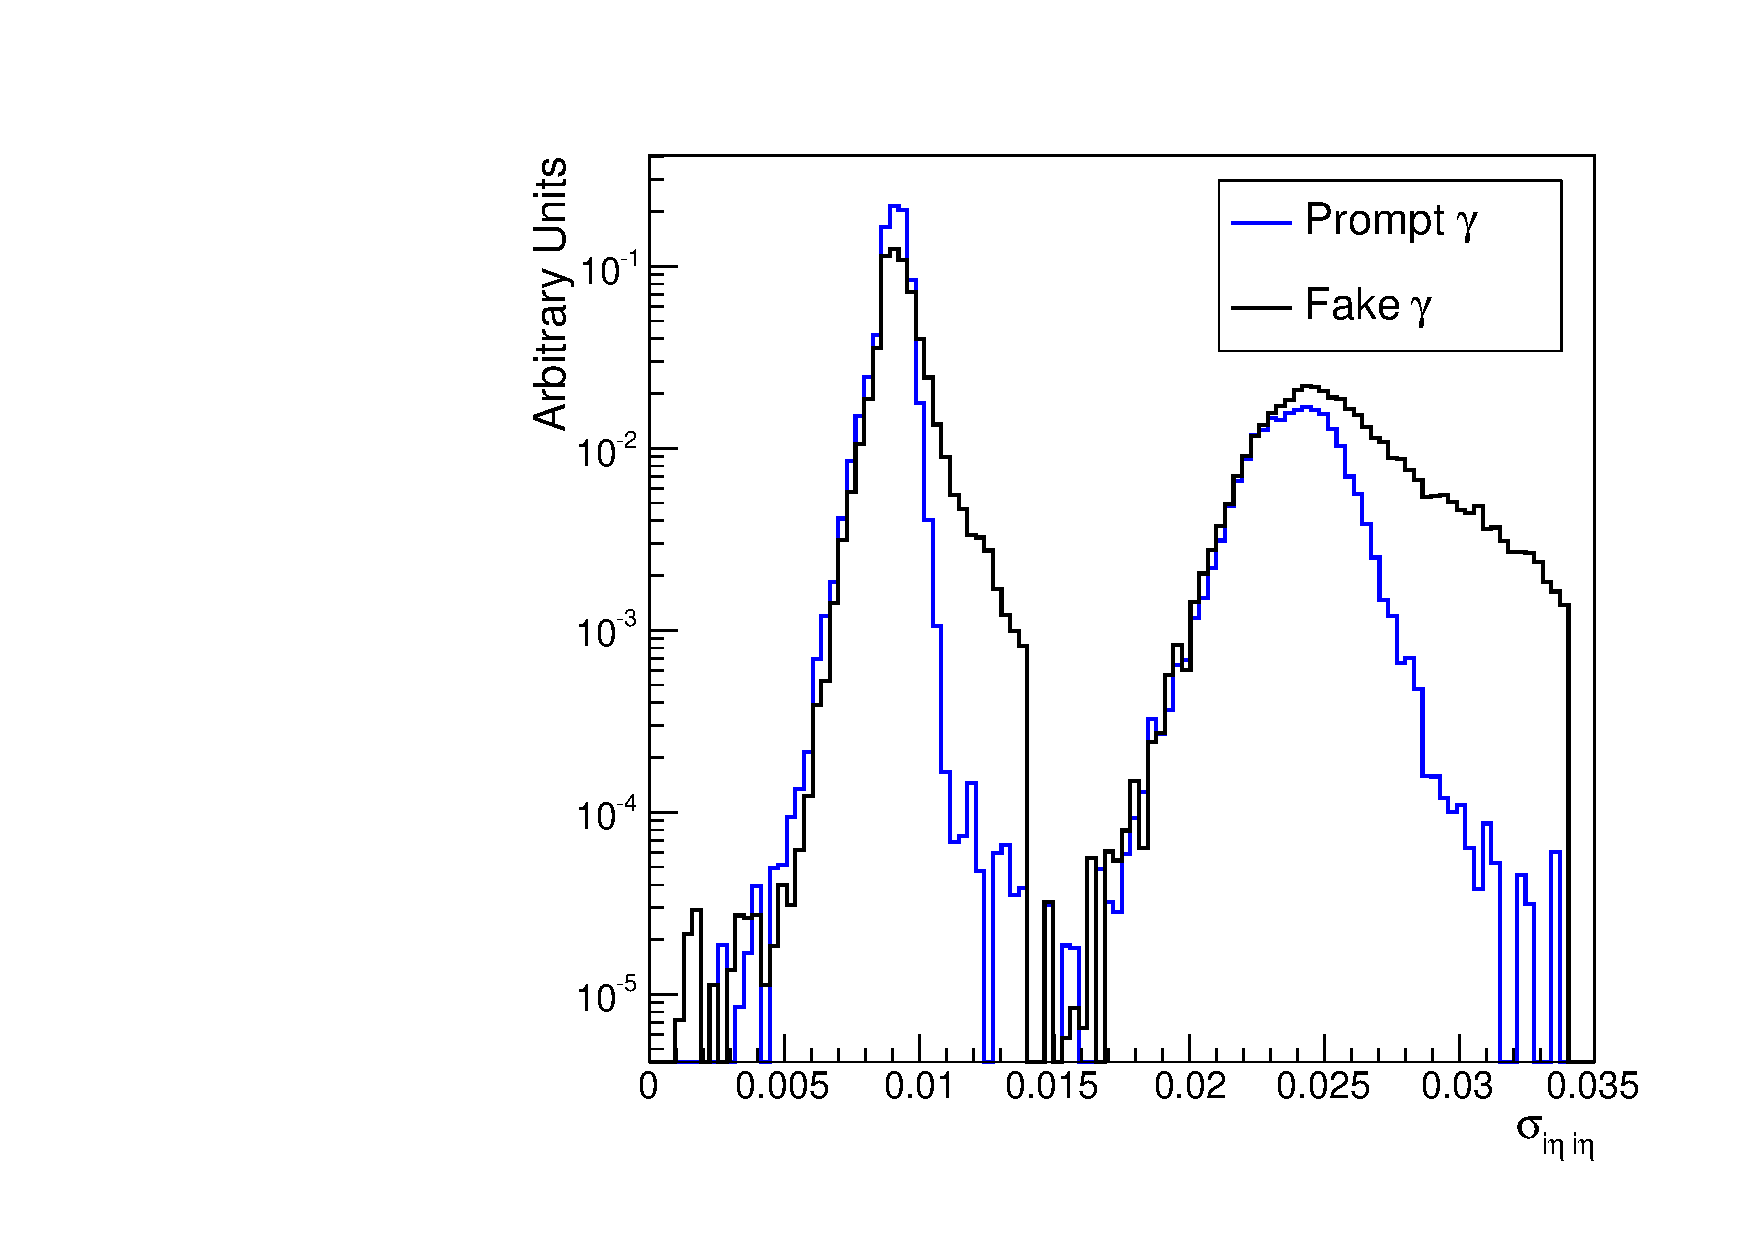
\includegraphics[width=0.49\textwidth]{detector/sieieeg.pdf}
	\caption{Shower shape variable $\rnine$ (left) and $\sigieie$ (right) distributions 
	for superclusters associated to simulated real and fake photons. The real photon is taken
	from simulated $\Hgg$ events while the fake photon is taken from a $\gamma+jet$ sample
	where the photon candidate is matched to a generated quark leg.}
	\label{fig:showershape}
\end{center}
\end{figure}

Hard interaction processes tend to produce electromagnetic particles which are well
isolated in the detector. A cone is defined around the candidate with radius $\Delta R$ defined as,
\begin{equation}
\Delta R = \sqrt{\Delta\phi^{2}+\Delta\eta^{2}}
\end{equation}
where $\Delta\phi$ and $\Delta\eta$ are positions relative the particle trajectory.
The sum of $E_{T}$ for each crystal inside the cone, after removing those associated 
to the supercluster itself, quantifies the isolation of the electron or photon candidate.
Similarly, such isolation variables exist for the HCAL and tracker detector elements,
summing over the $E_{T}$ and $p_{T}$ of HCAL deposits and tracks respectively,
are defined in an analogous way to the ECAL isolation.

